\documentclass[12pt]{article}
\usepackage{graphicx}
\usepackage{caption}
\usepackage{subcaption}
\usepackage{tikz}
\usepackage{venndiagram}
\usepackage{venndiagram}
\usepackage{tcolorbox}
\usepackage{listings}
\usepackage{enumitem}
\usepackage{amsmath}
\usepackage{amssymb}
\usepackage{colortbl}
\usepackage{xcolor}
\usepackage[margin=1cm, top=1.5cm, bottom=1.5cm]{geometry}

\tcbuselibrary{breakable}

\title{\textbf{Álgebra Superior I: Tarea 01}}
\author{Rendón Ávila Jesús Mateo}
\date{\today}

\begin{document}

\maketitle
\begin{center}
\vspace{3cm}
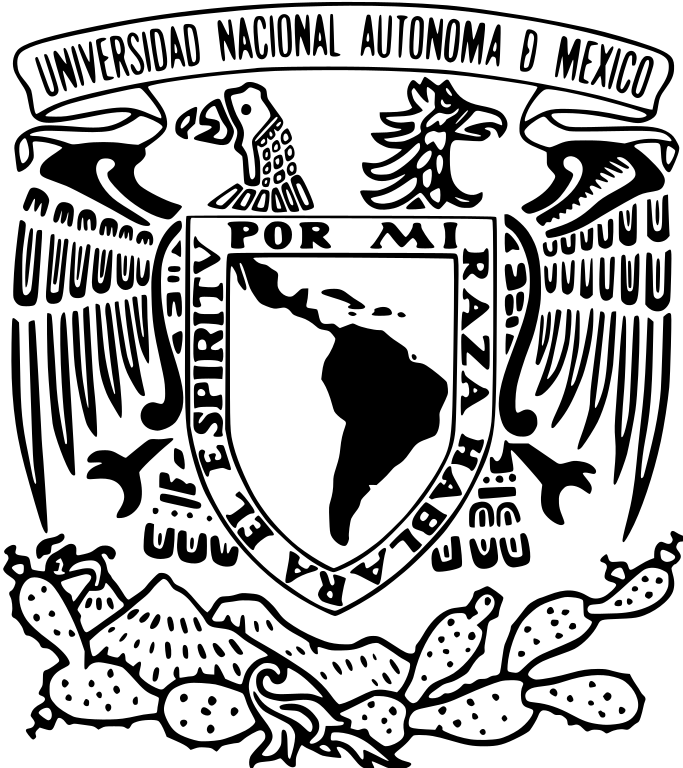
\includegraphics[width=0.195\textwidth]{Escudo.png}
\hspace{0.5cm}
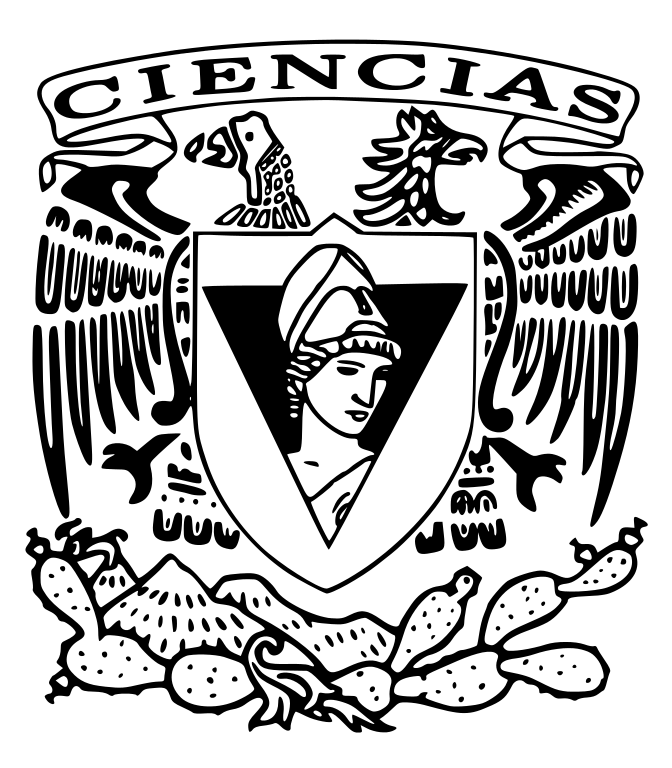
\includegraphics[width=0.2\textwidth]{logo_ciencias.png}
\end{center}
\begin{center}
    \vspace{1cm}
    Universidad Nacional Autónoma de México\\
    Facultad de Ciencias\\
    Profesora: Cristina Angélica Núñez Rodríguez\\
\end{center}

\newpage

%
% Ejercicio 1
%
\textbf{1.} Encuentra una proposición adecuada para describir a cada uno de los siguientes conjuntos.
\begin{enumerate}[label=\alph*)]
    \item $A = \{30, 31, 32, ...\}$\\
    $A = \{x \in \mathbb{N} \mid x \geq 30\}$
    \item $B = \{-1, 2, -3, 4, -5, 6, -7, ...\}$\\
    $B = \{x \in \mathbb{N}-\{0\} \mid \text{ si } x \mod 2 \neq 0 \Rightarrow -1(x)\}$
    \item $C = \{-1, 3, -5, 7, -9, 11, ...\}$\\
    $C = \{x \in \mathbb{N} - \{0\} \mid \text{ si } \}$
    \item $D = \{4, 7, 12, 19, ...\}$\\
    $D = \{...\}$
\end{enumerate}

%
% Ejercicio 2
%
\textbf{2.} Describe los siguientes conjuntos listando todos sus elementos.
\begin{enumerate}[label=\alph*)]
    \item $\{x \in \mathbb{N} \mid x^2 - 3x = 0\}$\\
    $\{3\}$

    \item $\{n^3 + n^2 \mid n \in \{0, 1, 2, 3, 4\}\}$\\
    $\{0, 2, 12, 36, 80\}$

    \item $\{\frac{1}{n^2 + n}\mid n \text{ es un positivo impar y } n \in \{1, 2, 3, 4, 5, 7\}\}$\\
    $\{\frac{1}{2}, \frac{1}{12}, \frac{1}{30}, \frac{1}{56}\}$

    \item $\{l \in \mathbb{Z} \mid l = 2n -1 \text{ y } -3 \leq n \leq 9\}$\\
    $\{-7, -5, -3, -1, 1, 3, 5, 7, 9, 11, 13, 15, 17\}$
\end{enumerate}

%
% Ejercicio 3
%
\textbf{3.} Sea $\mathbb{N}$ el conjunto de los números naturales. Determinar $ A \cup B$, $A \cap B$ y $A^c$ en:
\begin{enumerate}[label=\alph*)]
    \item $A = \{n \mid n \text{ es par}\}$ y $B = \{n \mid n < 14\}$\\
    $A \cup B = \{2, 4, 6, 8, 10, ...\}$\\
    $A \cap B = \{2, 4, 6, 8, 10, 12\}$\\
    $A^c = \{1, 3, 5, 7, 9, 11, ...\}$

    \item $A = \{n \mid n^2 > 2n - 1\}$, $B = \{n \mid n^2 = 2n + 3\}$\\
    $A \cup B =  \{2, 3, 4, 5, 6, ...\}$\\
    $A \cap B = \{9\}$\\
    $A^c = \{0, 1\}$
\end{enumerate}

%
% Ejercicio 4
%
\textbf{4.} Dibuja el diagrama de Venn para el siguiente problema:
\\

Un grupo de jóvenes fue entrevistado acerca de sus preferencias por diferentes medios
de transporte: bicicleta, motocicleta y automóvil. Los datos de las encuestas fueron los
siguientes:
\begin{itemize}
    \item Motocilceta solamente 5.
    \item Motocicleta 38.
    \item No gustan del automóvil 9.
    \item Motocicleta y bicicleta pero no automóvil 3.
    \item Motocicleta y automóvil pero no bicicleta 20.
    \item No gustan de la bicicleta 72.
    \item No gustan de las tres cosas 19.
    \item No gustan de la motocicleta 61.
\end{itemize}
Si tomamos al Conjunto $A$ como los que gustan de motocicleta, al $B$ los que gustan de 
bicicleta y al $C$ los que gustan de automóvil, entonces el diagrama de Venn es:
\begin{center}
    \begin{venndiagram3sets}[labelOnlyA={5},labelOnlyB={1},labelOnlyC={47},
        labelOnlyAB={3},labelOnlyAC={20},labelOnlyBC={13},labelABC={10},
        labelNotABC={19}]
    \end{venndiagram3sets}
\end{center}

Determinar: 

\begin{enumerate}[label=\alph*)]
    \item ¿Cuál fue el número de personas entrevistadas?\\
    118 personas
    \item ¿A cuántos les gusta la bicicleta solamente?\\
    una persona
    \item ¿A cuántos les gusta el automóvil solamente?\\
    47 personas
    \item ¿A cuántos les gustan las tres cosas?\\
    10 personas
    \item ¿A cuántos les gusta la bicicleta y el automóvil pero no la motocicleta?\\
    61 personas
\end{enumerate}

%
% Ejercicio 5
%
\textbf{5.} Sean $A$ y $B$ conjuntos. Prueba que:
\begin{enumerate}[label=\alph*)]
    \item $A - B = B^c - A^c$\\
    Demostraremos por propiedad de conjuntos:
    \begin{align*}
        A - B &= A \cap B^c \textit{( por propiedad de diferencia.)}\\
        &= B^c \cap A \textit{( por conmutatividad de intersección.)}\\
        &= B^c - A^c \textit{( por propiedad de diferencia.)}
    \end{align*}

    \item $B \subseteq A \Longleftrightarrow (A - B) \cup B = A$

    $\subseteq)$ Sea $x \in B$ por definición de subconjunto $x \in A$\\
    como $x \in A$ y $x \in B$ entonces $x \notin A - B$\\
    como $x \notin A - B$ y $x \in B$ entonces $x \in (A - B) \cup B$\\
    y por hipotesis, como $B \subseteq A$ entonces $B \cup (A - B) = A$\\
    \\
    $\supseteq)$ Sea $x \in (A - B) \cup B$ entonces\\
    $x \in A - B$ o $x \in B$\\
    como por nuestra hipotesis $(A - B) \cup B = A$ entonces $x \in A$\\
    por lo que debe ser $x \in A - B$
    como $x \notin B$ pero si $x \in (A - B) \cup B$ entonces debe ser $B \subseteq A$\\
    \\
    $\therefore B \subseteq A \Longleftrightarrow (A - B) \cup B = A$
\end{enumerate}

%
% Ejercicio 6 
%
\textbf{6.} Sean $A$, $B$ y $C$ tres conjuntos cualesquiera. Demuestra que:
\begin{enumerate}[label=\alph*)]
    \item $(A - B) - C = A - (B \cup C)$\\
    Demostraremos por propiedades de conjuntos:
    \begin{align*}
        (A - B) - C &= (A \cap B^c) - C\\
        &= (A \cap B^c) \cap C^c \textit{ (por propiedad de diferencia.)}\\
        &= A \cap (B^c \cap C^c) \textit{ (por leyes De Morgan)}\\
        &= A \cap (B \cup C)^c \textit{ (por propiedad de diferencia.)}\\
        &= A - (B \cup C)
    \end{align*}

    \item Si $A \subseteq B \Longrightarrow (A - C) \subseteq (B - C)$\\

    \textbf{Hipótesis}. $A \subseteq B$, entonces $x \in A \Longrightarrow x \in B$\\
    
    $PD$. $(A - C) \subseteq (B - C)$\\
    Sea $x \in A - C \Longrightarrow x \in A \land x \notin C$\\
    por hipotesis sabemos que $x \in B$ y por el paso anterior $x \notin C$\\
    así, $x \in B - C$\\
    de nuevo por nuestra hipótesis $A \subseteq B \Longrightarrow (A - C) \subseteq (B - C)$\\
    $\therefore$ si $A \subseteq B$ entonces $(A - C) \subseteq (B - C)$

\end{enumerate}

%
% Ejercicio 7
%
\textbf{7.} Sean $A$ y $B$ dos conjuntos. Definimos $A \bigtriangleup B = (A - B) \cup (B - A)$. Demuestra que:
\begin{enumerate}[label=\alph*)]
    \item $A \cap (B \bigtriangleup C) = (A \cap B) \bigtriangleup (A \cap C)$\\
    $\subseteq)$\\
    $P.D$. $A \cap (B \bigtriangleup C) \subseteq (A \cap B) \bigtriangleup (A \cap C)$
    sea $x \in A \cap (B \bigtriangleup C) \Longrightarrow x \in A \land x \in (B \bigtriangleup C)$\\
    por definición de $\bigtriangleup$ tenemos que $x \in A$ y  $x \in (B - C) \cup (C - B)$\\
    ahora, si $x \in (B - C) \cup (C - B) \Longrightarrow x \in B - C \lor x \in C - B$\\
    \\
    como tenemos una unión, entonces tenemos dos casos:
    \[\text{i) } x \in B - C \Longrightarrow x \in B \land x \notin C\]
    \[\text{ii) } x \in C - B \Longrightarrow x \in C \land x \notin B\]
    Si fuera i), entonces $x \in A$ y $x \in B$ y $x \notin C$\\
    $\Longrightarrow x \in A \cap B$ y $x \notin A \cap C$\\
    entonces $x \in (A \cap B) - (A \cap C)$\\
    con ello $x \in (A \cap B) \bigtriangleup (A \cap C)$\\
    \\
    Si fuera ii), entonces $x \in A$ y $x \in C$ y $x \notin B$\\
    $\Longrightarrow x \in A \cap C$ y $x \notin A \cap B$\\
    entonces $x \in (A \cap C) - (A \cap B)$\\
    con ello, por definición de $\bigtriangleup$, tenemos $x \in (A \cap B) \bigtriangleup (A \cap C)$\\
    \\
    Como en ambos casos $x \in (A \cap B) \bigtriangleup (A \cap C)$
    entonces $A \cap (B \bigtriangleup C) \subseteq (A \cap B) \bigtriangleup (A \cap C)$\\
    \\
    $\supseteq)$\\
    $P.D$. $(A \cap B) \bigtriangleup (A \cap C) \subseteq A \cap (B \bigtriangleup C)$


    \item Sean $A = \{a, b, c, d\}$, $B = \{3, 5, 7, c\}$ y $C = \{a, 1, 3, c\}$, encuentra:
    \begin{enumerate}
        \item $A \bigtriangleup B$\\
        $A \bigtriangleup B = (A - B) \cup (B - A) = \{a, b, d, 3, 5, 7\}$\\

        \item $A \cap (B \bigtriangleup C)$\\
        $B \bigtriangleup C = \{a, 1, 5, 7\}$\\
        $A \cap (B \bigtriangleup C) = \{a\}$\\

        \item $ B \bigtriangleup A$\\
        $B \bigtriangleup A = (B - A) \cup (A - B) = \{a, b, d, 3, 5, 7\}$
    \end{enumerate}
\end{enumerate}

%
% Ejercicio 8
%
\textbf{8.} Sean $A$, $B$, $C \subseteq \mathcal{U}$:
\begin{enumerate}[label=\alph*)]
    \item Expresa $(A - B)^c$ en terminos de $\cup$ y -:\\
    $(\mathcal{U} - A) \cup B$

    \item Demuestra que: $A - (B \cap C) = (A - B) \cup (A - C)$\\
    Demostraremos por propiedades de conjuntos:
    \begin{align*}
        A - (B \cap C) &= A \cap (B \cap C)^c \textit{ (por propiedad de la diferencia)}\\
        &= A \cap (B^c \cup C^c) \textit{ (por leyes De Morgan)}\\
        &= A - (B^c \cup C^c)^c \textit{ (por propiedad de diferencia.)}\\
        &= A - (B \cap C) \textit{ (por leyes De Morgan)}\\
        &= (A - B) \cup (A - C) \textit{ (por leyes De Morgan)}
    \end{align*}
\end{enumerate}

% 
% Ejercicio 9
%
\textbf{9.} Da un contraejemplo para probar la falsedad de los siguientes enunciados:

\begin{enumerate}[label=\alph*)]
    \item $A \cap (B \cup C) = A \cap C \Longrightarrow A \cap C = \varnothing$\\

    Proponemos los conjuntos:
    \[A = \{1, 2, 3, 4\}, B = \{7, 8, 9\} \text{ y } C = \{2, 5, 6, 7\}\]
    Primero determinaremos $B \cup C$, que es el conjunto $\{2, 5, 6, 7, 8, 9\}$. Ahora, $A \cap (B \cup C) = \{2\}$, notemos que:
    \[A \cap C = \{2\} \neq \varnothing\]
    cumpliendo la igualdad $A \cap (B \cup C) = A \cap C$ con $A \cap C \neq \varnothing$. Por lo tanto hemos exibido un elemento 
    que no cumple la proposición.

    \item $A - (B - C) = (A - B) - C$\\

    Proponemos los conjuntos:
    \[A = \{3, 4, 5, 9, 10, 11, 12\}, B = \{3, 4, 5, 6, a, b, c\} \text{ y } C = \{5, 6, 7, 8, 9\}\]
    Primero realizamos el conjunto $B - C$, que resulta ser $\{3, 4, a, b, c\}$. con el podemos realizar 
    el conjunto $ A - (B - C) = \{5, 9, 10, 11, 12\}$.\\

    Ahora podemos realizar el conjunto $A - B = \{9, 10, 11, 12\}$, de aquí podemos formar el 
    conjunto $(A - B) - C = \{10, 11, 12\}$\\

    Como es evidente $A - (B - C) \neq (A - B) - C$, los conjuntos propuestos prueban la falsedad de la proposición.
\end{enumerate}

%
% ejercicio 10
%
\textbf{10.} Sean $A$ y $B$ dos conjuntos. Demuestra que:

\begin{enumerate}[label=\alph*)]
    \item $A \subset B \Longleftrightarrow \mathcal{P}(A) \subset \mathcal{P}(B)$\\

    \textit{Hipotesis.} $A \subset B$, enotnces $\forall x \in A \Longrightarrow x \in B$\\

    Si tuvieramos $x \in A$, por nuestra hipotesis será $x \in B$.\\

    Por la definición de $\mathcal{P}(A)$ tenemos que $\mathcal{P}(A) = \{x \mid x \subseteq A\}$, y como sabemos $A \subset B$ entonces
    todo subconjunto de de $A$ es tambien subconjunto de $B$, así:
    \[\mathcal{P}(A) \subset \mathcal{P}(B)\]

    \item Si $A \cap B = \varnothing \Longrightarrow \mathcal{P}(A - B) = [\mathcal{P}(A) - \mathcal{P}(B)] \cup \{\varnothing\}$

    Si $A \cap B = \varnothing$ entonces $\forall x \in A \Longrightarrow x \notin B$ y $\forall z \in B \Longrightarrow z \notin A$\\

    $\subseteq)$\\
    $P.D$ $\mathcal{P}(A - B) \subseteq [\mathcal{P}(A) - \mathcal{P}(B)] \cup \{\varnothing\}$\\
    
    Como $A \cap B = \varnothing$, por la definición de \textit{diferencia de conjuntos} sabemos que se cumple $A - B = A$. De lo anterior 
    afirmamos que $ \mathcal{P}(A - B) = \mathcal{P}(A)$\\

    Como $A$ y $B$ son conjuntos disjuntos, entonces sus potencias $\mathcal{P}(A)$ y $\mathcal{P}(B)$ sólo comparten un 
    elemento que es el conjunto vacío $\varnothing$. Así:
    \[\mathcal{P}(A) - \mathcal{P}(B) = \mathcal{P}(A) - \{\varnothing\}\]
    De lo anterior tenemos $\mathcal{P}(A - B) \subseteq [\mathcal{P}(A) - \mathcal{P}(B)] \cup \{\varnothing\}$\\

    $\supseteq)$\\
    $P.D$ $[\mathcal{P}(A) - \mathcal{P}(B)] \cup \{\varnothing\} \subseteq \mathcal{P}(A - B)$\\

    Como sabemos por hipotesis que $A \cap B = \varnothing$ podemos deducir que $A - B = A$.\\

    De lo anteriro podemos decir:
    \[\mathcal{P}(A) - \mathcal{P}(B) = \mathcal{P}(A) - \{\varnothing\}\]
    \[(\mathcal{P}(A) - \{\varnothing\}) \cup {\varnothing} = \mathcal{P}(A)\]

    De nuevo por hipótesis sabemos que $A - B = A$, entonces $\mathcal{P}(A) = \mathcal{P}(A - B)$\\

    Así hemos demostrado que $[\mathcal{P}(A) - \mathcal{P}(B)] \cup \{\varnothing\} \subseteq \mathcal{P}(A - B)$\\

    $\therefore$ si $A \cap B = \varnothing \Longrightarrow \mathcal{P}(A - B) = [\mathcal{P}(A) - \mathcal{P}(B)] \cup \{\varnothing\}$

\end{enumerate}

%
% Ejercicio 13
%
\textbf{13.} Determina cuáles de las siguientes oraciones son proposiciones:

\begin{enumerate}[label=\alph*)]
    \item Algunos números enteros son negativos.\\
    Es una proposición con valor de verdad $V$.
    \item El número 15 es un número par.\\
    Es una proposición con valor de verdad $F$.
    \item ¿Qué hora es?\\
    No es una proposición pues no se puede determinar veracidad.
    \item En los números enteros, $11 + 6 \neq 12$\\
    Si es proposición con valor de verdad $V$.
    \item La tierra es casi una esfera.\\
    Si es una proposición con valor de verdad $V$.
\end{enumerate}

%
% Ejercicio 14
%
\textbf{14.} Si $P$ y $R$ representan proposiciones verdaderas y $Q$ y $S$ representan proposiciones falsas,
encuentra el valor de verdad de las proposiciones compuestas dadas a continuación:

\begin{enumerate}[label=\alph*)]
    \item $\neg P \land R$\\
    $F \land V = F$

    \item $\neg [\neg P \land (\neg Q \land P)]$\\
    $\neg[F \land (V \land V)] = \neg[F \land V] = \neg F = V$

    \item $(P \land R) \lor \neg Q$\\
    $(V \land V) \lor V = V \lor V = V$

    \item $P \Longrightarrow (Q \Longrightarrow R)$\\
    $V \Longrightarrow (F \Longrightarrow V) = V \Longrightarrow V = V$

    \item $[(P \land \neg Q) \Longrightarrow (Q \land R)] \Longrightarrow (S \lor \neg Q)$\\
    $[(V \land V) \Longrightarrow (F \land V)] \Longrightarrow (F \lor V) = [V \Longrightarrow F] \Longrightarrow V = F \Longrightarrow V = V$
\end{enumerate}

%
% Ejercicio 15
%
\textbf{15.} Responde:

\begin{enumerate}[label=\alph*)]
    \item Si la proposición $Q$ es verdadera, determine todas las asiganciones de valores de
    verdad para las proposiciones $P$, $R$ y $S$ para la proposición:
    \[\{Q \Longrightarrow [(\neg P \lor R) \land (\neg S)]\} \land \{\neg S \Longrightarrow (\neg R \land Q)\}\]
    
    Vamos a realizar una sola tabla para ahorra espacio:
    \begin{table}[h!]
        \centering
        \begin{tabular}{|c|c|c|c|||c|||c|c|c||c||c||||c||||c|||c|||c|c|c|}
            \hline
            $Q$ & $P$ & $R$ & $S$ & $\Longrightarrow$ & $\neg P$ & $\lor$ & $R$ & $\land$ & $\neg S$ & $\land$ & $\neg S$ & $\Longrightarrow$ & $\neg R$ & $\land$ & $Q$\\
            \hline
            V & V & V & V & F & F & V & V & F & F & F & F & V & F & F & V\\
            V & V & V & F & V & F & V & V & V & V & F & V & F & F & F & V\\
            V & V & F & V & F & F & F & F & F & F & F & F & V & V & V & V\\
            V & V & F & F & F & F & F & F & F & V & F & V & V & V & V & V\\
            V & F & V & V & F & V & V & V & F & F & F & F & V & F & F & V\\
            V & F & V & F & V & V & V & V & V & V & F & V & F & F & F & V\\
            V & F & F & V & F & V & V & F & F & F & F & F & V & V & V & V\\
            V & F & F & F & V & V & V & F & V & V & V & V & V & V & V & V\\
            F & V & V & V & V & F & V & V & F & F & V & F & V & F & F & F\\
            F & V & V & F & V & F & V & V & V & V & F & V & F & F & F & F\\
            F & V & F & V & V & F & F & F & F & F & V & F & V & V & F & F\\
            F & V & F & F & V & F & F & F & F & V & F & V & F & V & F & F\\
            F & F & V & V & V & V & V & V & F & F & V & F & V & F & F & F\\
            F & F & V & F & V & V & V & V & V & V & F & V & F & F & F & F\\
            F & F & F & V & V & V & V & F & F & F & V & F & V & V & F & F\\
            F & F & F & F & V & V & V & F & V & V & F & V & F & V & F & F\\
            \hline           
        \end{tabular}
        \caption{Tabla de valor de las variables}
    \end{table}
    
\end{enumerate}

\end{document}